\chapter{Astronomy, Optics and Telescopes}
\thispagestyle{fancy}
\begin{multicols}{2}
A \textbf{parsec}\index{Parsec} is defined so
\begin{align}
1 \textrm{ parsec}=\frac{1\textrm{ AU}}{\tan(1")} \approx \frac{1\textrm{ AU}}{1"}
\end{align}
The \textbf{flux}\index{Flux} ($F$) of a star relates to it's luminosity ($L$) and distance ($d$) via
\begin{align}
F  &= \frac{L}{4\pi R^2} = \sigma_{SB} T_{eff}^4
\end{align}
The flux received by a telescope at distance d is then
\begin{align}
	F(d)  &= \frac{L}{4\pi d^2} = \sigma T_{eff}^4\left(\frac{R}{d}\right)^2
\end{align}
The ratio of two magnitudes using different filters from a single star gives a rough estimation of the stars color.
\begin{align}
B-V&=m_B-m_V=-2.5\log_{10}\bigg(\frac{F_B}{F_V}\bigg) \\
\frac{F_B}{F_V}&=10^{-(M_B-M_V)/2.5}
\end{align}
We define the \textbf{distance modulus}\index{Distance modulus} ($DM$) as the difference in apparent magnitude ($m$) between a given star and the absolute magnitude ($M$) it would have if it were at 10 pc.
\begin{align}
DM &\equiv m-m(10 \textrm{ pc}) \equiv m-M \\
M &\equiv m-DM
\end{align}
The full form of intensity as a function of angle from the beam axis is
\begin{align}
I=I_0\bigg[\frac{\sin(\pi D/\lambda \sin(\theta))}{\sin(\pi d/\lambda \sin(\theta))} \bigg]^2
\end{align}
Snell's Law: 
\begin{align}
\frac{\sin(\theta_1)}{\sin(\theta_2)} = \frac{v_1}{v_2} = \frac{\lambda_1}{\lambda_2}=\frac{n_2}{n_1}
\end{align}






\section{Celestial Orbits}
Suppose we have a exoplanet system with a planet $p$ and a star $s$. The vector from the star to the planet is $\vec{r}_{sp}=\vec{r}_p-\vec{r}_s$, and the force that the star exerts on the planet is ($\vec{r}_n$ is the vector from the origin to $n$)
\begin{align}
\vec{F}_{sp}=-\frac{GM_pM_s}{|\vec{r}_{sp}|^3}\vec{r}_{sp}
\end{align}
If we put the origin at the center of mass ($\vec{R}$ is the vector from the origin to the center of mass)
\begin{align}
\vec{R}=\frac{M_s\vec{r}_s+M_p\vec{r}_p}{M_s+M_p}
\end{align}
Then the star and planets have positions
\begin{align}
\vec{x}_s &= \vec{r}_s-\vec{R}=-\frac{M_p}{M_p+M_s}\vec{r}_{sp} \\
\vec{x}_p &= \vec{r}_p-\vec{R}=-\frac{M_s}{M_p+M_s}\vec{r}_{sp} 
\end{align}
And thus accelerations
\begin{align}
\frac{d^2\vec{x}_s}{dt^2} &=-\frac{M_p}{M_p+M_s}\frac{d^2 \vec{r}_{sp}}{dt^2} \\
\frac{d^2\vec{x}_p}{dt^2} &=-\frac{M_s}{M_p+M_s}\frac{d^2 \vec{r}_{sp}}{dt^2} 
\end{align}
Substituting the acceleration into the equation of motion for the planet,
\begin{align}
M_p\frac{d^2 \vec{x}_p}{dt^2}=\vec{F}_{sp}
\end{align}
Then we can get the reduced equation of motion as
\begin{align}
\frac{d^2 \vec{r}_{sp}}{dt^2}=-G\frac{M_s+M_p}{|\vec{r}_{sp}|^3}\vec{r}_{sp}
\end{align}
Keplar's Third law: The solution to this is an elliptical orbit with the center-of-force at one focus of the ellipse. The period ($T$) depends on the semi-major axis ($a$)
\begin{align}
T^2=\frac{4\pi^2}{G(M_s+M_p)}a^3 \\
a^3=\frac{G(M_s+M_p)}{4\pi^2}T^2
\end{align}
If the orbit is circular, so that $|\vec{r}_sp=a$ is constant, then the orbital speed of the star is
\begin{align}
v_s=\frac{2\pi aM_p}{T(M_p+M_s)}=\sqrt{\frac{GM_p^2}{a(M_p+M_s)}}
\end{align}
For a particle in a circular orbit, $v = r\Omega \hat{\theta}$; using Kepler’s law (r is the distance from the center of mass), we have
\begin{align}
L=mr^2\Omega = m\sqrt{GMr}.
\end{align}
The orbital angular momentum of the two-body system is
\begin{align}
L&=\frac{M_1M_2}{M_1+M_2} a^2\Omega\\
&= \frac{M_1M_2}{M_1+M_2}\sqrt{G(M_1+M_2)a}.
\end{align}
The angular momentum of a sphere is
\begin{align}
L=\frac{8\pi}{15}\rho\Omega R^5=\frac{2}{5}MR^2\Omega.
\end{align}
The equations of motion in a rotating frame are
\begin{align}
\frac{d^2\vec{r}'}{dt^2}&=\frac{1}{m}\vec{F}_{rot} \\
&=\frac{1}{m}\vec{F}+\underbrace{r\Omega^2\hat{r}}_\text{centrifugal}+\underbrace{2\Omega(v_\theta\hat{r}-v_r\hat{\theta})}_\text{coriolis}.
\end{align}
Particles within a sphere of radius $R_H$ are dominated by the gravitational attraction of $M_2$; $R_H$ (the Hill radius) is
\begin{align}
R_H\approx a\bigg[\frac{M_2}{3(M_1+M_2)} \bigg]^{1/3}.
\end{align}





\section{Celestial \& Stellar Atmospheres}
The equation of hydrostatic equilibrium\index{Hydrostatic equilibrium}
\begin{align}
\frac{dP}{dr}=-\rho g.
\end{align}
The ideal gas law can be written (with $m$=mass of 1 mole of our gas) as 
\begin{align}
P=\bigg(\frac{mN/N_A}{V} \bigg)\frac{kN_A}{m}T\equiv \rho \frac{kN_A}{m}T.
\end{align}
Combining the above two equations and assuming $T$=constant then yields a relation between pressure and height as
\begin{align}
\frac{dP}{P}=-\frac{mg}{N_AkT}dz.
\end{align}
This then gives a pressure Dependant on height as
\begin{align}
P(z)=P_0\exp\bigg[-\frac{mgz}{N_AkT} \bigg].
\end{align}

In addition to the Coriolis acceleration from the Earth rotation, horizontal pressure gradients will also produce an acceleration
\begin{align}
-\frac{1}{\rho}\nabla P.
\end{align}
The equation for force and acceleration along r$\hat{r}$ is therefore
\begin{align}
\underbrace{\frac{v^2}{r}}_\text{centripital}+\underbrace{2v\Omega \sin(\lambda)}_\text{coriolis}-\underbrace{\frac{1}{\rho}\frac{dP}{dr}}_\text{pressure}=0.	
\end{align}
If matter is in thermal equilibrium, then populations of a two different
states of a given atom are given by Boltzmann’s formula\index{Boltzmann’s formula},
\begin{align}
	\frac{n_i}{n_j}=\frac{g_i}{g_j}exp\left(\frac{E_j-E_i}{kT}\right).
\end{align}
Hydrostatic equilibrium (where $m$ is the mass within a sphere of radius $r$, $P$ is the pressure, and $\rho$ is the mass density) gives two equations of stellar structure,
\begin{align}
	\frac{dm}{dr} &= 4\pi r^2 \rho \andspace{0.5cm}
	\frac{dP}{dr} = -\rho \frac{Gm}{r^2}
\end{align}
From the virial theorem, the average pressure and density are
\begin{align}
	\bar{\rho} &= \frac{GM}{4\pi R^3} \andspace{0.5cm}
	\bar{P} \propto \frac{GM^2}{R^4}
\end{align}
The optical depth for an outward-directed ray is
\begin{align}
	\tau_\mu = \int_z^\infty\rho \kappa_\mu dz' \implies \frac{d\tau}{dz}=-\rho \kappa
\end{align}
From this, an estimate of the photospheric pressure can be determined  for a gray atmosphere in LTE\footnote{Local Thermodynamical Equilibrium} by,
\begin{align}
	\frac{dP}{d\tau} = -\left(\frac{d\tau}{dz}\right)^{-1}\rho g = \frac{g}{\kappa}.
\end{align}
From hydrostatic equilibrium and taking $\rho=constant$ (where $\mu m_u$ is the average mass of a particle in the plasma), the central pressure and temperature are given by
\begin{align}
	T_c &=\frac{GM\mu m_u}{2Rk_B} \\
	P_c &= \frac{3GM^2}{8\pi R^4}
\end{align}
Bringing a small amount of mass $dm$ from infinity onto a sphere of mass m and radius r gives a potential change of
\begin{align}
	d\Omega = -\frac{Gm}{r}dm.
\end{align}
For a constant density, we have $r=R(m/M)^{1/3}$ and so
\begin{align}
	\Omega = -\frac{3GM^2}{5R}.
\end{align}
Using this, the mean temperature and pressure for a constant density sphere is
\begin{align}
	\bar{T} &= \frac{GM\mu m_u}{5Rk_B} \\
	\bar{P} &= \frac{3GM^2}{20\pi R^4}.
\end{align}
The free fall time it would take for a star to collapse if all internal pressures were removed is \begin{align}
	\tau_{ff} = \frac{\pi}{\sqrt{GM}}\left(\frac{R}{2}\right)^{3/2} = \left(\frac{3}{32\pi}\right)^{1/2}\frac{1}{\sqrt{G\bar{\rho}}}.
\end{align}
The \textbf{dynamical timescale}\index{Dynamical timescale} of the star is defined from the proportionality constant of the free fall time
\begin{align}
	t_{dyn} \equiv \frac{1}{\sqrt{G\bar{\rho}}}.
\end{align}
Any change in pressure is communicated through a star by sound waves which travel at the speed
\begin{align}
	c_s = \left(\gamma \frac{P}{\rho}\right)^{1/2}=\left(\gamma \frac{k_BT}{\mu m_u}\right)^{1/2}.
\end{align}
The time it takes for a sound wave to travel a distance R is then
\begin{align}
	\tau_{sc} = \frac{R}{c_s} = \sqrt{\frac{3R^3}{GM}} = \left(\frac{3}{2\sqrt{\pi}}\right)\frac{1}{\sqrt{G\bar{\rho}}}.
\end{align}
The \textbf{Kelvin-Helmholtz timescale} is the time it would take the sun to radiate all of it's gravitational energy away with it's current luminosity $L_\odot$,
\begin{align}
	t_{KH} \approx \frac{GM_\odot^2}{R_\odot L_\odot} \approx 3 \times 10^7 yr.
\end{align}
{\centering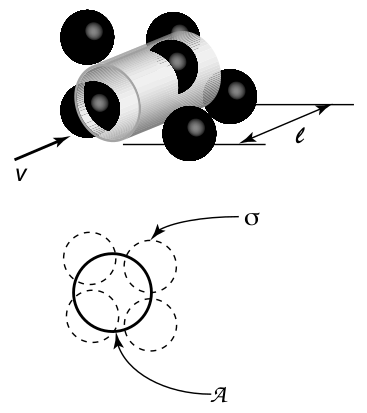
\includegraphics[width=0.8\columnwidth]{./Images/Diagrams/meanfreepath.png}}\\
As displayed by the image above\footnote{"Schematic of a particle incident on a group of particles." \cite{bib:AST304}.}, the probability of a particle making it through a density of obstacles $n$ with cross section $\sigma$ is
\begin{align}
	\mathcal{P} = \frac{n(\mathcal{A}\ell)\sigma}{\mathcal{A}} = n\sigma \ell.
\end{align}
The \textbf{mean free path} is defined to be the length at which $\mathcal{P}\rightarrow 1$ which is when the particle will suffer a collision:
\begin{align}
\ell = \frac{1}{n\sigma}.
\end{align}


\section{Convection}
The temperature gradient in a star ($\kappa= opacity$) is
\begin{align}
\frac{dT}{dr} = -\frac{3\rho\kappa}{4acT^3}\frac{L(r)}{4\pi r^2}.
\end{align}
From the first law of thermodynamics,
\begin{align}
dQ &= dU - \frac{P}{\rho^2}d\rho \\
dU &=  \left(\frac{\partial U}{\partial T}\right)_\rho dT +\left(\frac{\partial U}{\partial \rho}\right)_T d\rho \\
dQ &= \left(\frac{\partial U}{\partial T}\right)_\rho dT +\left[\left(\frac{\partial U}{\partial \rho}\right)_T- \frac{P}{\rho^2}\right] d\rho.
\end{align}
While holding density fixed, the heat needed to raise the temperature of one kilogram of fluid is then
\begin{align}
C_\rho \equiv \left(\frac{\partial Q}{\partial T}\right)_\rho = \left(\frac{\partial U}{\partial T}\right)_\rho.
\end{align}
From this, heat transfer can be expressed as a function of temperature and pressure
\begin{align}
dQ &= \left[C_\rho+\frac{P}{\rho T}\right]dT - \frac{1}{\rho}dP \\
&= \left[C_\rho+\frac{k_B}{\mu m_u}\right]dT - \frac{1}{\rho}dP.
\end{align}
Hence, while holding pressure fixed, the heat needed to raise the temperature of one kilogram of fluid is
\begin{align}
C_P = \left(\frac{\partial Q}{\partial T}\right)_P = C_\rho + \frac{k_B}{\mu m_u}.
\end{align}
For a plasma of ions and electrons,
\begin{align}
C_\rho =\frac{3k_B}{2\mu m_u} = \frac{3}{5} C_P.
\end{align}
Thus the ratio of specific heats for an ideal gas is
\begin{align}
\gamma = \frac{C_P}{C_\rho} = \frac{5}{3}.
\end{align}
During adiabatic motion, no heat exchange occurs and so $TdS = dQ =0$ which leads to
\begin{align}
T=T_0\left(\frac{P}{P_0}\right)^{(\gamma -1)/\gamma}.
\end{align}
The temperature change with pressure in an adiabatically stratified gas is given by
\begin{align}
\frac{P}{T}\left(\frac{\partial T}{\partial P}\right)_S = \left(\frac{\partial \ln T}{\partial \ln P}\right)_S = \frac{\gamma -1}{\gamma}.
\end{align}
For stable convection, we must have
\begin{align}
\left(\frac{\partial V}{\partial S}\right)_P\frac{dS}{dr} = \frac{T}{C_P}\left(\frac{\partial V}{\partial T}\right)_P\frac{dS}{dr} > 0.
\end{align}
The stability requirements for convection can also be derived in terms of local gradients of temperature and pressure. The fluid is unstable to convection if
\begin{align}
\frac{P}{P_{rad}}\frac{\kappa}{16\pi Gc}\frac{L(r)}{m(r)} > \left(\frac{\partial \ln T}{\partial \ln P}\right)_S = \frac{\gamma-1}{\gamma}.
\end{align}
\section{Main Sequence Stars}
For an enclosed mass we have the following relations for radiative and convective regions respectively
\begin{align}
	\frac{dT}{dr} &= -\frac{L}{4\pi r^2}\frac{3\rho \kappa}{4acT^3} \\
	\frac{dT}{dr} &= \frac{T}{P}\left(\frac{\partial \ln T}{\partial \ln P}\right)_S \frac{dP}{dr}.
\end{align}
The fourth order equation of stellar structure  (with $\epsilon$ being the heating rate per unit mass) is
\begin{align}
	\frac{dL}{dr} = 4\pi r^2\rho \epsilon.
\end{align}
\end{multicols}

\section{Galaxies}

The Friedmann-Lema\^{i}tre-Robertson-Walker (FLRW) Metric which relates space and time and is an exact solution of Einsteins field equations in general relativity using the assumptions of homogeneous and isotropic space ($a(t)$ is the expansion parameter).
\begin{align}
	c^2 \textrm{ds}^2=-c^2\textrm{dt}^2+a(t)^2\left(\frac{dr^2}{1-(r/r_0)^2}+r^2(\textrm{d}\theta^2+\sin^2\theta \textrm{d}\phi^2) \right) = -c^2\textrm{dt}^2+\textrm{d}\vec{\Sigma}^2
\end{align}
From this, we can determine a flux-luminosity relation that is dependent upon the expansion parameter.
\begin{align}
	F_\nu(\nu)=\frac{L(\nu a^{-1})a}{4\pi r(a)^2}.
\end{align}
We can define a density parameter for each type of matter as
\begin{align}
	\Omega_i = \frac{8\pi G \rho_i}{3H^2}.
\end{align}

